\section*{Math 202a - HW6 - Dan Davison - \texttt{ddavison@berkeley.edu}}

\begin{mdframed}
  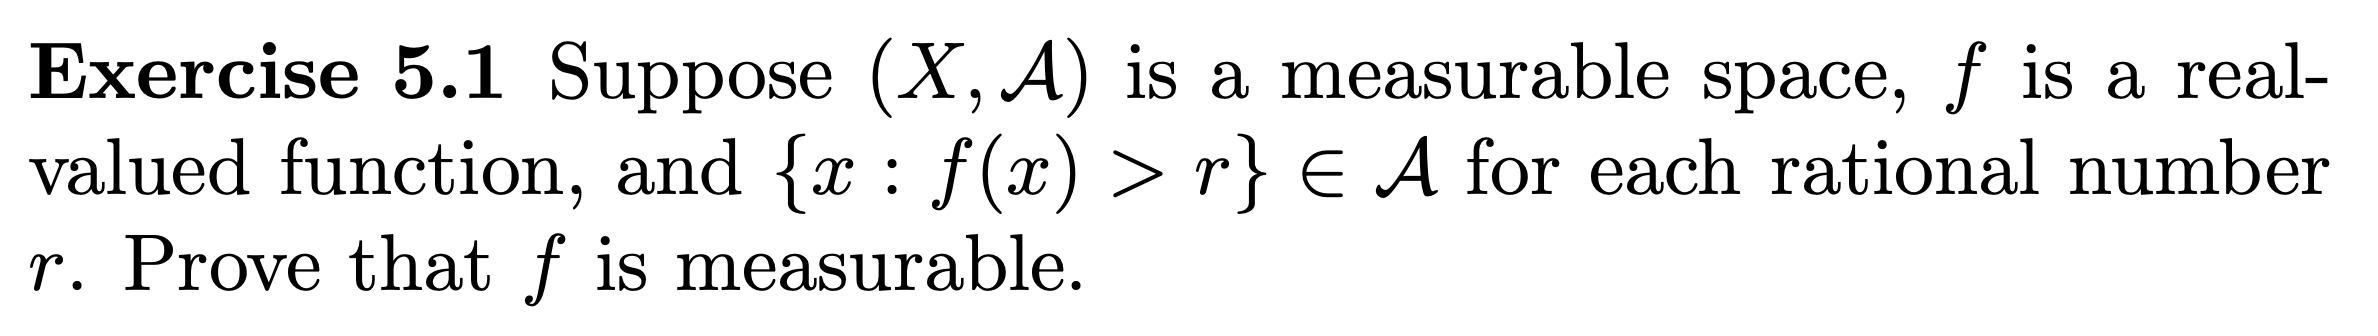
\includegraphics[width=400pt]{img/analysis--berkeley-202a-hw06-ab56.png}
\end{mdframed}

\begin{proof}
  Let $a \in \R$. Define $q_i$ to be the number formed by truncating the decimal expansion of $a$ at the $i$-th
  digit. Then $q_1, q_2, \ldots \in \Q$ is a sequence of rationals with $\lim_{i \to \infty} q_i = a$. Therefore
  \begin{align*}
    \lim_{i \to \infty} \{x ~:~ f(x) > q_i\} = \{x ~:~ f(x) > a\},
  \end{align*}
  and hence
  \begin{align*}
    \{x ~:~ f(x) > a\} = \bigcup_{i=1}^\infty \{x ~:~ f(x) > q_i\}.
  \end{align*}
  Therefore $\{x ~:~ f(x) > a\}$ is a countable union of elements of $\mc A$, for all $a \in \R$. Therefore $f$
  is $\mc A$-measurable.
\end{proof}



\newpage
\begin{mdframed}
  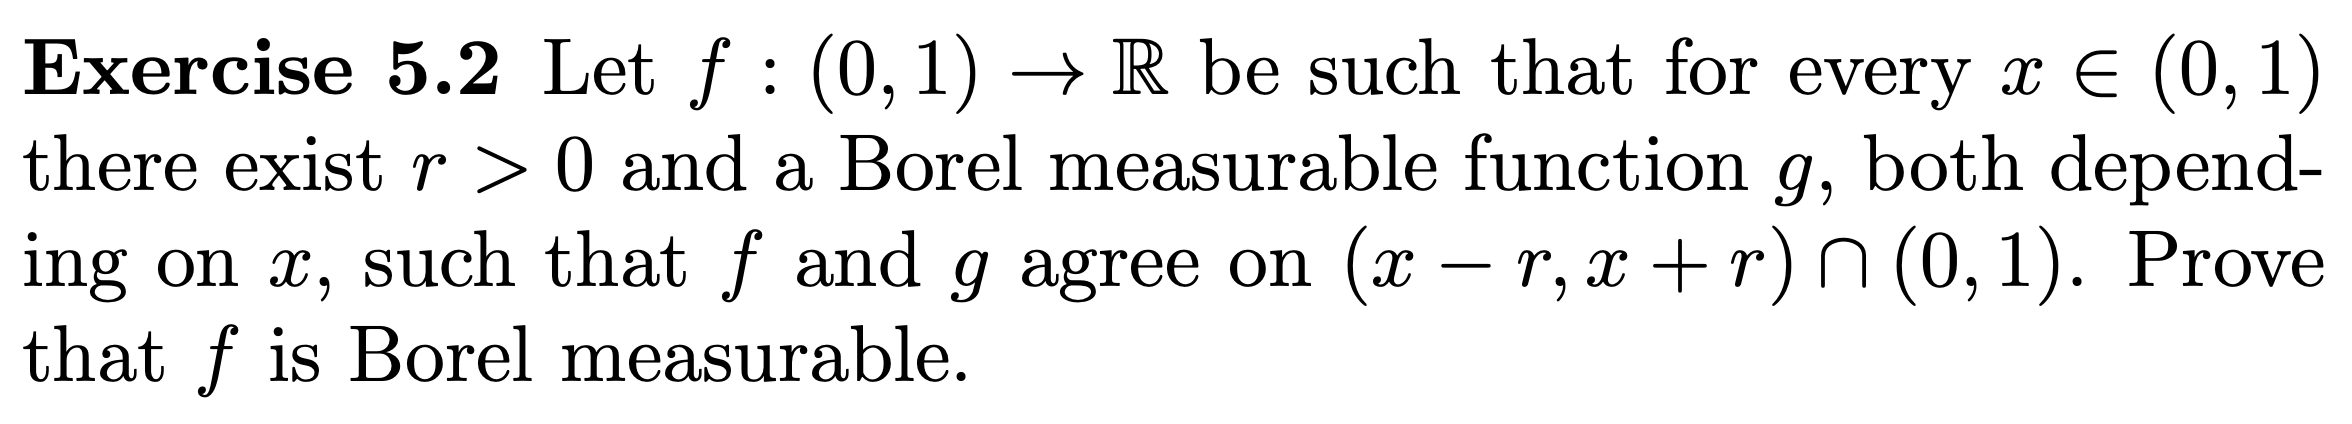
\includegraphics[width=400pt]{img/analysis--berkeley-202a-hw06-927a.png}
\end{mdframed}

\begin{proof}
  Let $\mc A$ be the Borel $\sigma$-algebra on $(0, 1)$ and for every $x \in (0, 1)$ let $r_x > 0$ be such
  that $f$ and $g_x$ agree on $(x - r_x, x + r_x) \cap (0, 1)$, and $g_x$ is Borel-measurable.

  We must show that $\{x ~:~ f(x) > y\} \in \mc A$ for all $y \in \R$.

  Let $y \in \R$ and let $q_1, q_2, \ldots \in \Q \cap (0, 1)$ be an enumeration of the rationals in $(0, 1)$.

  Define $U_{a} := \{x ~:~ g_{a}(x) > y\} \cap (a - r_{a}, a + r_{a})$. Note that $U_a$ is a set of real
  numbers $x$ near $a$ for which we know that $f(x) > y$.

  We claim that $\{x ~:~ f(x) > y\} = \bigcup_{i=1}^\infty U_{q_i} \in \mc A$.

  Let $w = \inf \{r_{q_i} ~:~ i \in \N \}$.

  To prove the forwards inclusion, let $b \in \{x ~:~ f(x) > y\}$, and let $q \in (b - w, b + w) \cap \Q$. Note
  that $b \in (q - r_q, q + r_q)$ and therefore $g_q(b) = f(b) > y$. Therefore $b \in U_q$, proving the
  forwards inclusion.

  To prove the reverse inclusion, let $b \in \bigcup_{i=1}^\infty U_{q_i}$. Then $b \in U_q$ for
  some $q \in \{q_1, q_2, \ldots\}$. Therefore $f(b) > y$.

  Finally, note that $U_a$ is the intersection of two Borel-measurable sets and hence is Borel-measurable.
  Therefore $\bigcup_{i=1}^\infty U_{q_i}$ is Borel-measurable.
\end{proof}

\newpage
\begin{mdframed}
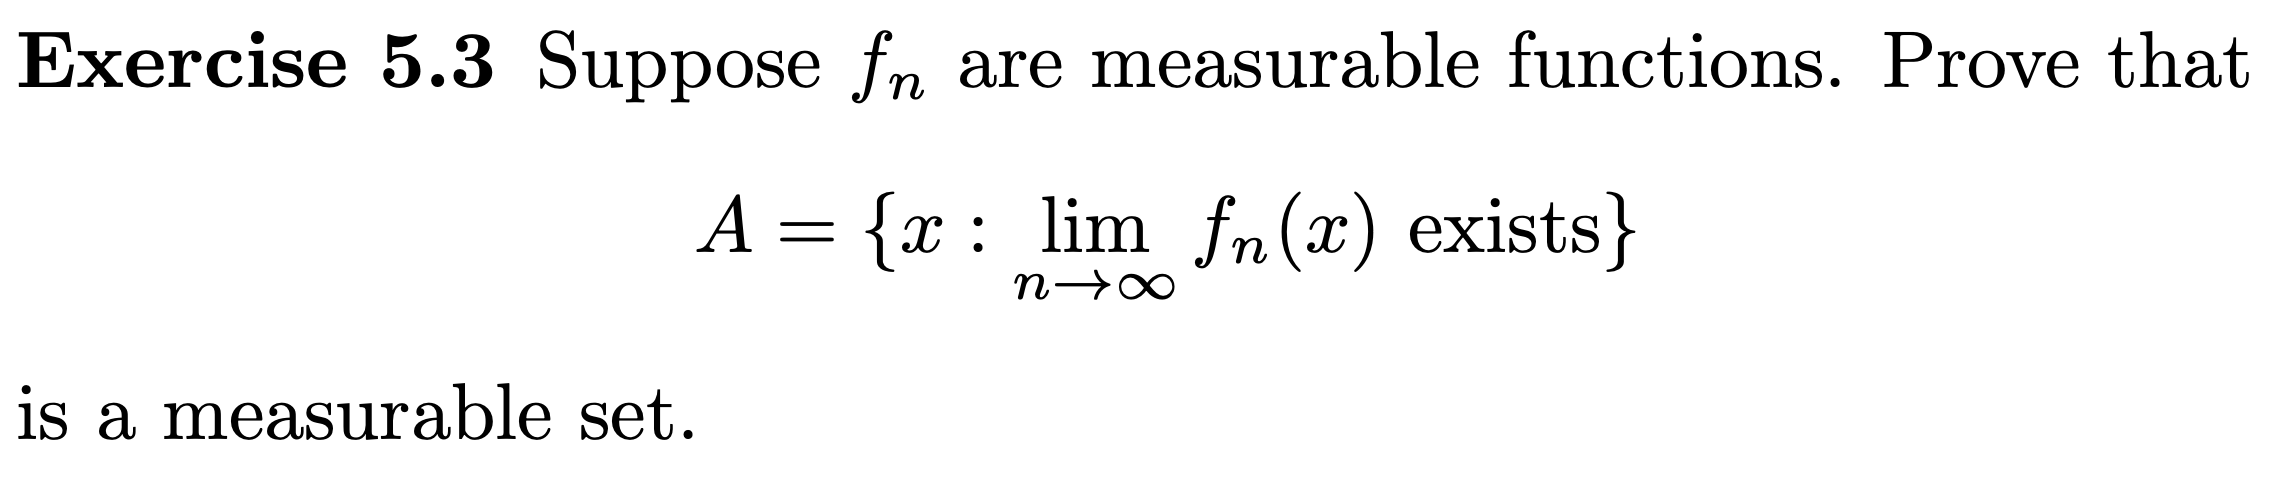
\includegraphics[width=400pt]{img/analysis--berkeley-202a-hw06-aaf5.png}
\end{mdframed}

\begin{proof}

  (Incomplete)

  We know that the preimage under $f_n$ of an open set is measurable.

  We want to show that $A$ is measurable. We will do that by showing that it is the preimage of an open set.

  $\lim_{n \to \infty} f_n(x)$ exists if there exists $y$ such that for all $\eps$ there exists $N$ beyond
  which $f_n(x)$ lies within $\eps$ of $y$.
\end{proof}

Sadly I was able to do this question's predecessor, but not the question I was supposed to be doing! FWIW,
here's the predecessor:

\begin{mdframed}
  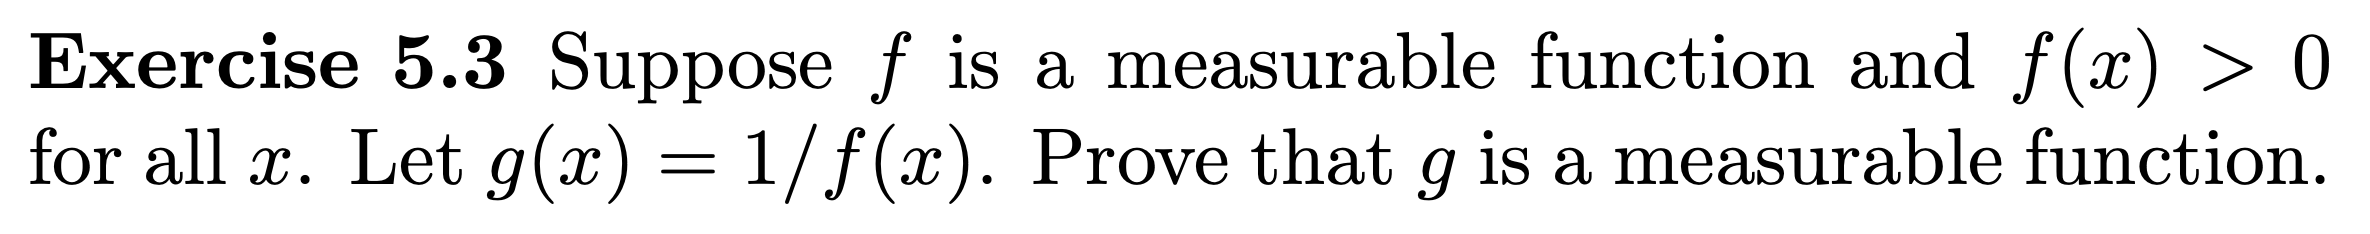
\includegraphics[width=400pt]{img/analysis--berkeley-202a-hw06-b799.png}
\end{mdframed}

\begin{proof}
  Let $f: X \to (0, \infty)$ be a measurable function, and let $g(x) = 1/f(x)$.

  Since $f$ is measurable, there exists a $\sigma$-algebra $\mc A$ such that $f^{-1}((y, \infty)) \in \mc A$
  for all $y > 0$.

  Let $h(x) = 1/x$. Then $g = h \circ f$.

  Fix $y \in (0, \infty)$ and let $U = h^{-1}((y, \infty)) \subseteq (0, \infty)$. Since $h$ is
  continuous, $U$ is open.

  We want to show that $g^{-1}((y, \infty)) \in \mc A$. We have
  \begin{align*}
    g^{-1}((y, \infty)) = f^{-1}(h^{-1}((y, \infty))) = f^{-1}(U).
  \end{align*}
  So what we want to show is that $f^{-1}(U) \in \mc A$, where $U \subseteq (0, \infty)$ is open.

  Write $U = \bigcup_{i=1}^\infty (a_i, b_i)$ where $(a_1, b_1), (a_2, b_2), \ldots \subseteq (0, \infty)$ is a
  countable pairwise disjoint collection of open intervals.

  Note that $f^{-1}(U) = \bigcup_{i=1}^\infty f^{-1}((a_i, b_i))$.

  Note also that $(a, b) = (a, \infty) \setminus (b, \infty)$ and therefore
  that $f^{-1}((a, b)) = f^{-1}((a, \infty)) \setminus f^{-1}((b, \infty))$.

  Thus we have
  \begin{align*}
    f^{-1}(U)
    &= \bigcup_{i=1}^\infty \Big(f^{-1}((a, \infty)) \setminus f^{-1}((b, \infty))\Big) \\
    &= \bigcup_{i=1}^\infty \Big(f^{-1}((a, \infty)) \cap \big(f^{-1}((b, \infty))\big)^c\Big) \\
    &\in \mc A,
  \end{align*}
  since this is a countable union of intersections of two sets that are both in $\mc A$ (one by definition, and
  one as the complement of a set that is in $\mc A$ by definition).
\end{proof}



\newpage
\begin{mdframed}
  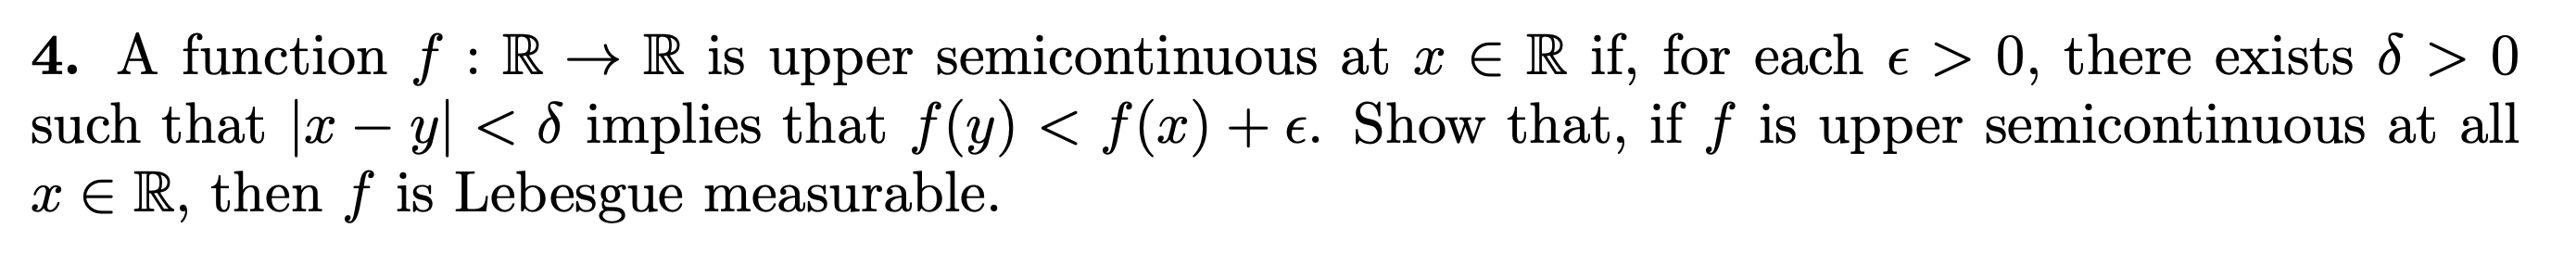
\includegraphics[width=400pt]{img/analysis--berkeley-202a-hw06-90b1.png}
\end{mdframed}


\begin{proof}
  It suffices to show that $f^{-1}\((-\infty, y)\)$ is open for all $y \in \R$, since
  then $f^{-1}\((-\infty, y)\)$ is Borel-measurable, and therefore Lebesgue-measurable.

  % We know that there is a theorem concerning continuous functions on metric/topological spaces: $f:\R \to \R$
  % is
  % continuous if and only
  % if $f^{-1}(U)$ is open for every open subset $U \subseteq \R$.

  % We want to prove the reverse direction of this, but assuming upper semicontinuity only. In other words, we
  % want to prove that (upper semicontinuity) implies (preimage of $(-\infty, q)$ is open) for all $q \in \R$.

  % We follow the proof of the standard theorem (see Kevin McGerty's Oxford A2 Metric Spaces notes) but
  % substituting upper semicontinuity.

  So, fix $y \in \R$ and let $a \in f^{-1}\((-\infty, y)\)$. It suffices to show that $f^{-1}\((-\infty, y)\)$
  includes a neighborhood of $a$, since then it contains a neighborhood of all its points and therefore is
  open as required.

  Since $f$ is upper semicontinuous there exists $\eps > 0$ and $\delta > 0$ such
  that $(a - \delta, a + \delta) \subset f^{-1}\((-\infty, f(a) + \eps)\)$.

  Note that $f(a) \in (-\infty, y)$.
  Therefore $(a - \delta, a + \delta) \subset f^{-1}\((-\infty, y + \eps)\)$.

  Since $\eps$ is arbitrary we have that $(a - \delta, a + \delta) \subseteq f^{-1}\((-\infty, y)\)$, and
  therefore that $f^{-1}\((-\infty, y)\)$ includes a neighborhood of $a$, as required.
\end{proof}

\newpage
\begin{mdframed}
  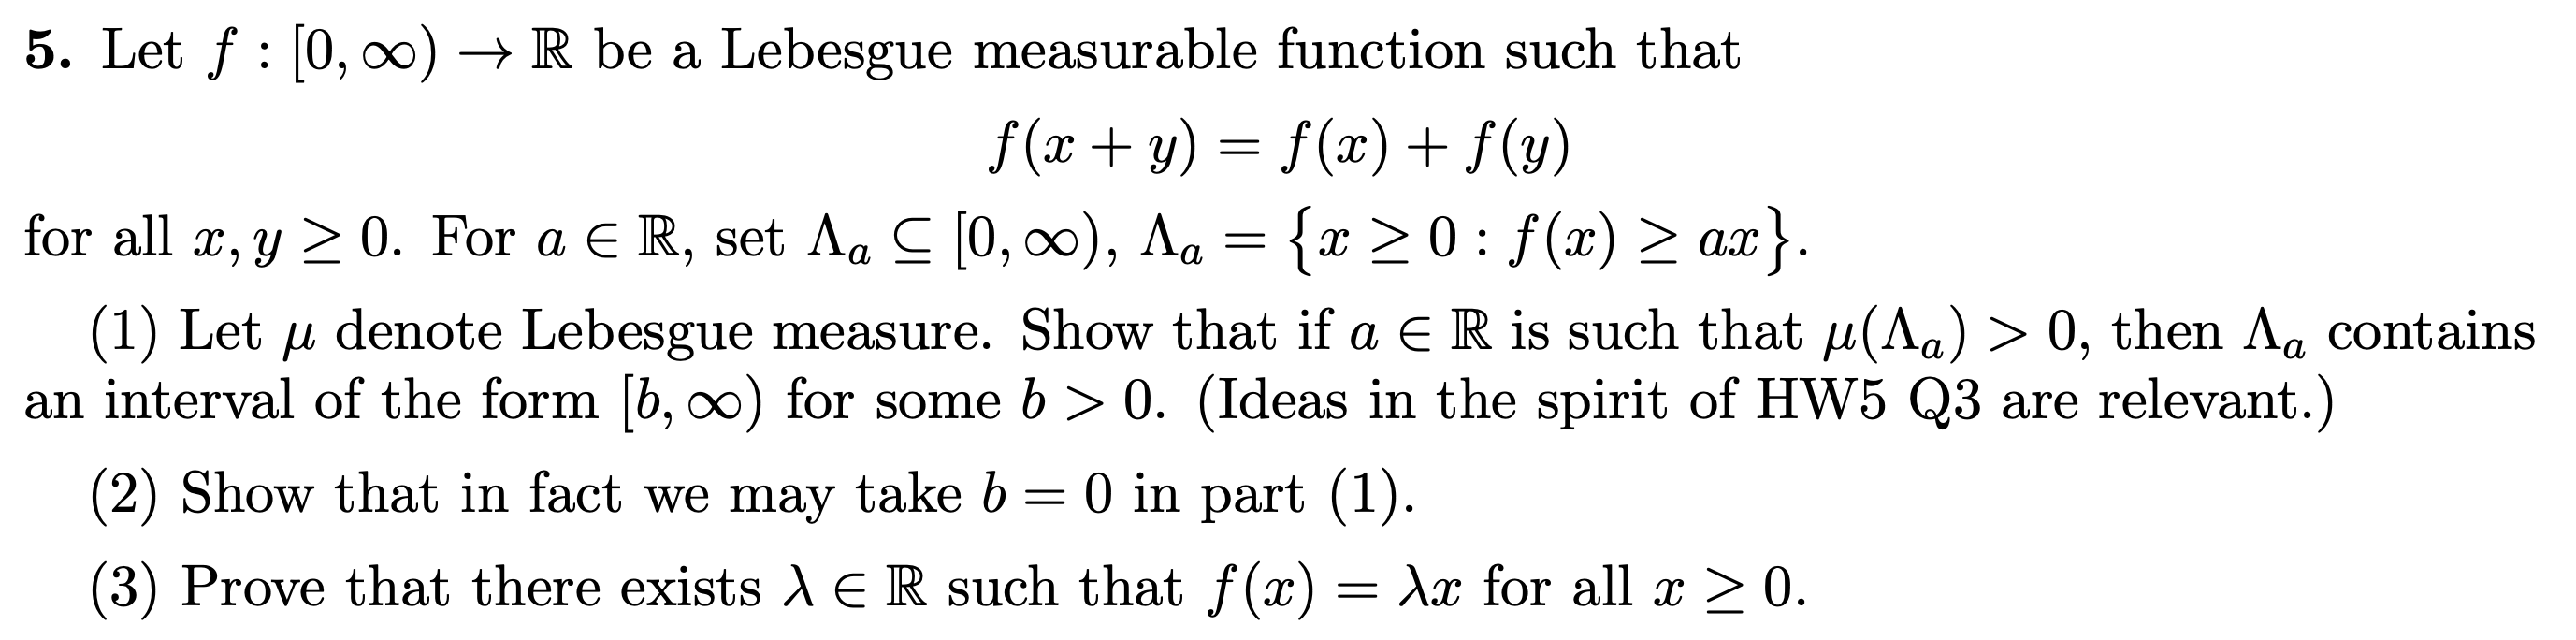
\includegraphics[width=400pt]{img/analysis--berkeley-202a-hw06-7769.png}
\end{mdframed}

Note that $f(0) = 0$, since $f(0) = f(0 + 0) = 2f(0)$, of which the only solution is $f(0) = 0$.

For $a \in \R$ define $g_a(x) := f(x) - ax$ so that $\Lambda_a = \{x \geq 0 ~:~ g_a(x) \geq 0\}$.

Note that $g_a$ is measurable for all $a \in \R$, and therefore $\Lambda_a$ is Lebesgue measurable for
all $a \in \R$. To see this, for $a \in \R$ define $h_a(x) = -ax$ so that $g_a = f + h_a$. Then $h_a$ is
clearly Lebesgue measurable for all $a \in \R$, and therefore so also is $g_a(x)$ (by Bass proposition 5.7
which states that a function produced via elementary operations on measurable functions is measurable).

\begin{proof}
  Fix $\eps > 0$ and let $I = (a, a + \eps)$.

  Note that $\{y - y' ~:~ y, y' \in I\} = (-\eps, \eps)$.

  Note also that $f^{-1}(y' - y) = f^{-1}(y') - f^{-1}(y)$. To see this, note
  that $f^{-1}(y) + \big[f^{-1}(y') - f^{-1}(y)\big] = f^{-1}(y')$. Therefore we have
  \begin{align*}
    f\Big(f^{-1}(y) + \big[f^{-1}(y') - f^{-1}(y)\big]\Big) &= f\big(f^{-1}(y')\big) \\
    f\Big(f^{-1}(y)\Big) + f\Big(\big[f^{-1}(y') - f^{-1}(y)\big]\Big) &= f\big(f^{-1}(y')\big) \\
    f\Big(\big[f^{-1}(y') - f^{-1}(y)\big]\Big) &= y' - y \\
    f^{-1}(y') - f^{-1}(y) &= f^{-1}(y' - y).
  \end{align*}

  Therefore
  \begin{align*}
    f^{-1}((-\eps, \eps))
    &= \Big\{f^{-1}(y - y') ~:~ y, y' \in I\Big\} \\
    &= \Big\{f^{-1}(y) - f^{-1}(y') ~:~ y, y' \in I\Big\} \\
    &= \Big\{x - x' ~:~ x, x' \in f^{-1}(I)\Big\}.
  \end{align*}
  Since $f^{-1}(I)$ we have from HW5 Q3 that there exists $\delta > 0$ such
  that $(-\delta, \delta) \subseteq f^{-1}((-\eps, \eps))$.

  Therefore $f$ is continuous.

  (3) Since $f$ is additive and continuous, it follows that it is linear.

  (1), (2) follow from (3).
\end{proof}




\newpage
\begin{mdframed}
  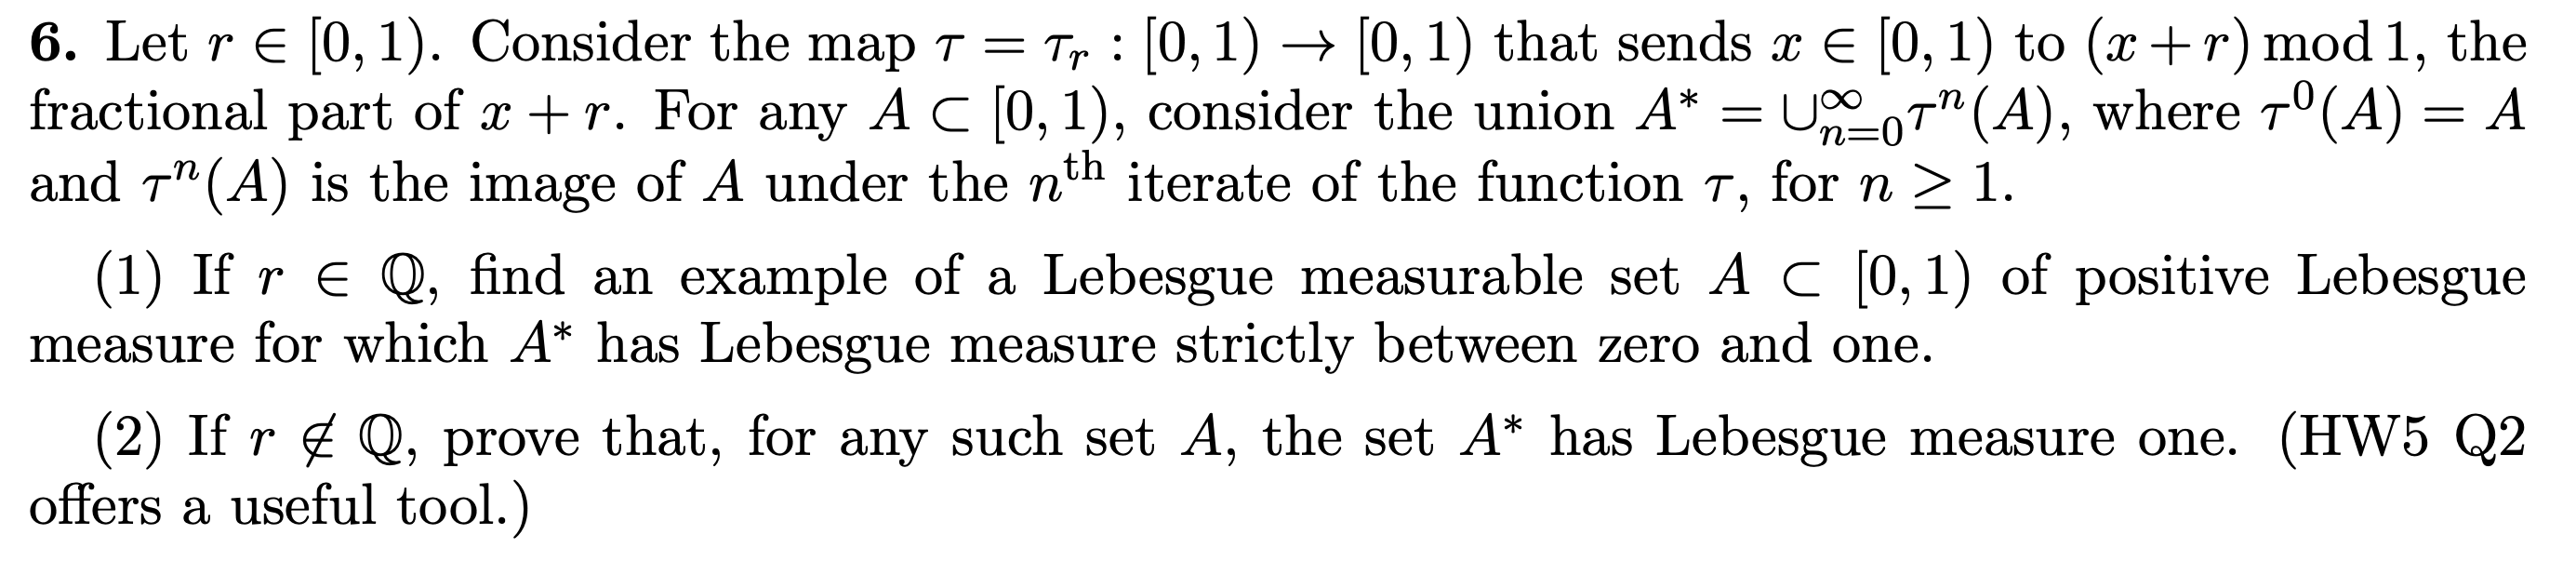
\includegraphics[width=400pt]{img/analysis--berkeley-202a-hw06-9bc5.png}
\end{mdframed}

\begin{intuition*}
  A point is in $A^*$ if it is reached starting from any point in $A$.

  A point is in $(A^*)^c$ iff it is never reached, starting from any point in $A$.

  If any point in $A$ reaches all points of the circle, then $\mu(A^*) = 1$.
\end{intuition*}

\begin{lemma*}
  Let $E \subseteq \R$ be Lebesgue measurable and fix $\alpha \in (0, 1)$. Then there exists an open
  interval $I_i$ such that $\mu(E \cap I_i) > \alpha \mu(I_i)$.
\end{lemma*}

Let $\mu$ denote Lebesgue measure.

Note that, since $\tau_r$ is a translation on the circle, it follows from translation-invariance of measure
that $\tau_r$ is a measure-preserving transformation, i.e. that
\begin{align*}
  \mu(\tau_r^{-1}(A)) = \mu(A).
\end{align*}

Let $\Omega = [0, 1)$. Then $(\Omega, \mu, \tau_r)$ is a dynamical system.

\begin{enumerate}
\item
  \begin{claim*}
    Let $r \in [0, 1) \cap \Q$. Then there exists $A \subset [0, 1)$ of positive Lebesgue measure such that $0 < \mu(A^*) < 1$.
  \end{claim*}
  \begin{proof}
    Let $r = p/q \in \Q$, where $p, q \in \Z$ are coprime.

    Let $I_i = [\frac{i}{2q}, \frac{i+1}{2q})$ and define $A = \bigcup_{i=0}^{2q-1} I_i$. We claim that $A$ has
    the required properties.

    Clearly $A$ has positive measure, since $\mu(A) = q \cdot \frac{1}{2q} = \frac{1}{2}$.

    Next we need to show that $0 < \mu(A^*) < 1$, where $A^* := \bigcup_{n=0}^\infty \tau^n(A)$.

    Informally, what we want to show is that the $I_i$ map to each other under $\tau$.

    We have
    \begin{align*}
      \tau^n(I_i)
      &= \Big[\big(\frac{i}{2q} + \frac{np}{q}\big) \mod 1, \big(\frac{i+1}{2q} + \frac{np}{q}\big) \mod 1 \Big) \\
      &= \Big[\frac{i + 2np}{2q} \mod 1, \frac{i + 1 + 2np}{2q} \mod 1\Big) \\
      &= \Big[\frac{(i + 2np) \mod 2q}{2q}, \frac{(i + 1 + 2np) \mod 2q}{2q}\Big) \\
      &= I_{(i + 2np) \mod 2q} \\
      &\subseteq A.
    \end{align*}
    Therefore $A^* := \bigcup_{n=0}^\infty \tau^n(A) \subseteq A$ and
    hence $\mu(A^*) \leq \mu(A) = \frac{1}{2}$. Since $A = \tau^0(A) \subset A^*$ we have
    \begin{align*}
      0 < \mu(A^*) < 1,
    \end{align*}
    as required.
  \end{proof}

\item

\begin{mdframed}
  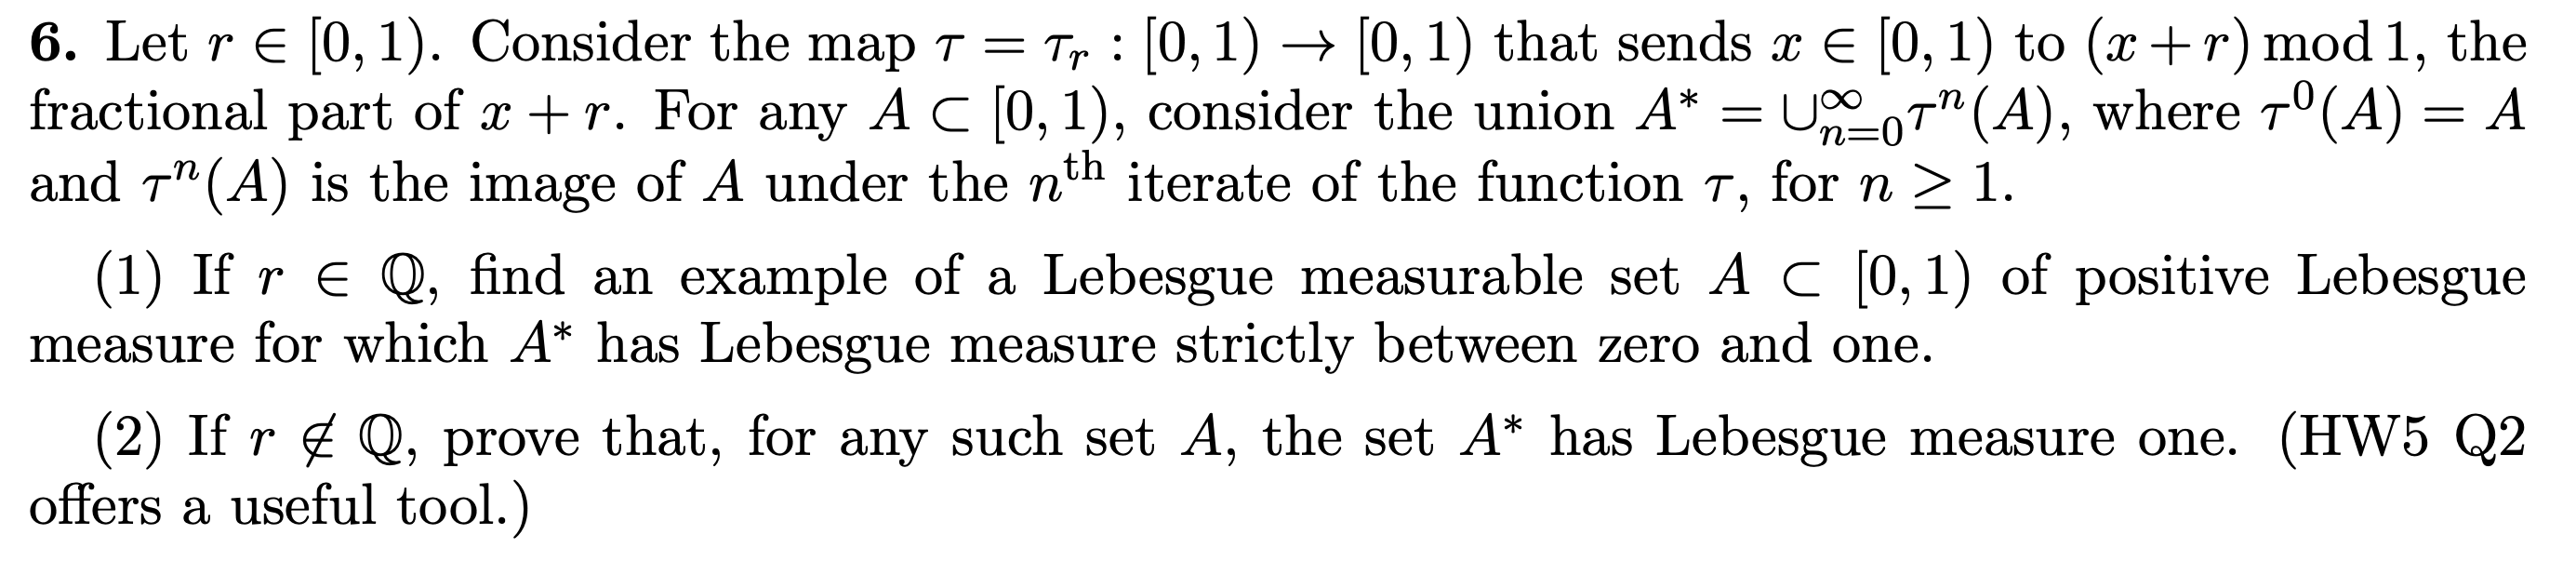
\includegraphics[width=400pt]{img/analysis--berkeley-202a-hw06-9bc5.png}
\end{mdframed}

  \begin{claim*}
    Let $r \in [0, 1) \setminus \Q$. Then $\mu(A^*) = 1$ for all $A \subset [0, 1)$.
  \end{claim*}

  \begin{intuition*}
    If $A$ includes an interval then the result is true. Furthermore, the result is intuitively plausible
    if $A$ does not include an interval​, as follows. We know that $A$ includes a locally dense region; the
    iterations of the dynamical system place many copies of this dense region around the circle such that every
    point of the circle is close to infinitely many copies of the dense region, each translated by small
    amounts from each other. Thus it is certainly plausible that the amount of space left uncovered is
    negligible.
  \end{intuition*}

  \begin{proof}
    Let $r \in [0, 1) \setminus \Q$ and let $A \subseteq [0, 1)$ have positive measure.

    For any subset $X \subseteq [0, 1)$ let $X^* \subseteq [0, 1)$ denote the union $\bigcup_{n=0}^\infty \tau^n(X)$.

    We will show that $\mu\((A^*)^c\) = 0$.

    Note that
    \begin{align*}
      \big(A^{*}\big)^c = \bigcap_{n=0}^\infty \big(\tau^n(A)\big)^c.
    \end{align*}
    Let $\eps > 0$.

    Then there exists an open interval $I$ such that $\mu(A \cap I) > (1 - \eps) \mu(I)$, or equivalently
    \begin{align*}
      \mu(I \setminus A) < \eps\mu(I).
    \end{align*}

    Let $d = \mu(I)$, and fix an arbitrary interval $J \subset [0, 1)$ of length $d$.

    We will show that $\mu(J \setminus A^*) < \epsilon d$. Since $J$ is an arbitrary interval, it follows that

  \end{proof}



  \begin{proof}
    Let $r \in [0, 1) \setminus \Q$ and let $A$ be a $\tau_r$-invariant set with positive measure.

    First suppose $A$ includes an interval $I$. Then $A^* = [0, 1)$. This is true because (a) the orbits are
    dense, so for any given point $x \in [0, 1)$ we can find $x_0 \in A$ whose orbit passes close to $x$. Then
    (b) we can look at how close it got, and find another starting point in our interval whose orbit hits $x$
    exactly.

    Suppose $A$ includes an interval $I = (a, b)$. We claim that $A^* = [0, 1)$.

    Proof: Let $y \in [0, 1)$ and let $\eps < \mu(I)$. Since $\orb(a)$ is dense, there exists $x \in \orb(a)$
    such that $|x - y| < \eps$.


    Now suppose $A$ includes no interval. We want to show that $\mu(A^*) = 1$.

    For any subset $X \subseteq [0, 1)$ let $X^*$ denote the union $\bigcup_{n=0}^\infty \tau^n(X)$.

    Since $I$ is an interval, we have $I^* = [0, 1)$ and $\mu(I^*) = 1$.

    We claim that $\mu((A \cap I)^*) = 1$. This implies the desired result
    since $(A \cap I)^* \subseteq A^* \subseteq [0, 1)$.

    Let $\eps > 0$.

    Then there exists an open interval $I$ such that $\mu(A \cap I) > (1 - \eps) \mu(I)$, or equivalently:
    \begin{align*}
      \mu(I \setminus A) < \eps\mu(I).
    \end{align*}

    Recall that we want to show that $\mu((A \cap I)^*) = 1$.

    We have the non-disjoint union
    \begin{align*}
      I^* = (A \cap I)^* \cup (I \setminus A)^*.
    \end{align*}
    Therefore
    \begin{align*}
      \mu(I^*) = 1 \leq
    \end{align*}



    Therefore we have $\mu(A \cap I) = \mu(I) - \mu(I \setminus A) > (1 - \eps)\mu(I)$,




    We know that $\mu(\tau^k(A \cap I)) > (1 - \eps)\mu(I)$ by translation invariance.






    We want to show that

    We must use
    \begin{enumerate}
    \item $\mu(A^*) > 0$ -- this gives the interval theorem
    \item Every point has a non-periodic orbit which is dense
    \item Orbits are disjoint
    \item $A^*$ is invariant: $\tau(A^*) = A^*$
    \end{enumerate}

    We want to show that the set of points we don't hit exactly has measure $0$.


  \end{proof}

  \begin{lemma}
    Every $\tau_r$-invariant set with positive measure has Lebesgue measure one when $r$ is irrational.
  \end{lemma}
  \begin{proof}
    Let $r \in [0, 1) \setminus \Q$ and let $A$ be a $\tau_r$-invariant set with positive measure.

    First suppose $A$ includes an interval $I$. Then $A^* = [0, 1)$. This is true because (a) the orbits are
    dense, so for any given point $x \in [0, 1)$ we can find $x_0 \in A$ whose orbit passes close to $x$. Then
    (b) we can find another orbit that hits $x$ exactly.


    Now suppose $A$ includes no interval. We need to show that the set of points we don't hit exactly has
    measure 0.

    We must use
    \begin{enumerate}
    \item $A$ is invariant: $\tau(A) = A$
    \item $\mu(A) > 0$
    \item Every point has a non-periodic orbit which is dense
    \item Orbits are disjoint
    \end{enumerate}

    Then for all $\eps > 0$ there exists an open interval $I$ such that $\mu(A \cap I) > (1 - \eps) \mu(I)$.



  \end{proof}

  \begin{proof}
    Let $r \in [0, 1) \setminus \Q$ and let $A \subset [0, 1)$ have positive Lebesgue measure.

    Note that $A^*$ has positive measure since $A = \tau^0(A) \subset A^*$ hence $\mu(A) < \mu(A^*)$. Note also
    that $A^*$ is invariant under $\tau$, since
    \begin{align*}
      \tau^{-1}(A^*)
      &:= \{x ~:~ \tau(x) \in A^* \} \\
      &= \{x ~:~ \tau(x) \in \bigcup_{n=0}^\infty \tau^n(A) \} \\
      &= \bigcup_{n=0}^\infty \tau^n(A) \\
      &=: A^*.
    \end{align*}




  \end{proof}
\end{enumerate}





    One option would be to prove that $\tau_r$ is ergodic with respect to Lebesgue measure. Then,
    since $\tau^{-1}(A^*) = A^*$ we have that $\mu(A^*) = 0$ or $\mu(A^*) = 1$.
    But $A = \tau^0(A) \subset A^*$, therefore $\mu(A^*) \neq 0$. Therefore $\mu(A^*) = 1$.





    Then every point has a non-periodic orbit which is dense in $[0, 1)$.


    Let $A \subset [0, 1)$ have positive measure.


    Recall that every point in the circle has a periodic orbit when $r$ is rational.




    Let $f:[0, 1) \to \C$ be defined by $f(x) = e^{2\pi ixq}$.

    Note that $f$ is invariant under $\tau_r$, since we have
    \begin{align*}
      f(\tau_r(x)) =
      \begin{cases}
        e^{2\pi i (x + p/q)q} = e^{2\pi i (qx + p)} = e^{2\pi iqx}e^{2p\pi i} = f(x)  ~~~~~~~~~~~~~~~~~~~~~x + a < 1, \\
        e^{2\pi i (x + p/q - 1)q} = e^{2\pi i (qx + p - q)} = e^{2\pi iqx}e^{2(p - q)\pi i} = f(x)  ~~~~~~~~x + a \geq 1.
      \end{cases}
    \end{align*}
    Informally, $f$ is the location of a point that is moving around the unit circle with constant
    velocity $q$.

    Since $\tau_r$ is not ergodic for rational $r$,
